\documentclass[sigconf]{acmart}

\usepackage{booktabs} % For formal tables
\usepackage{amsmath}
\usepackage{bm}
\usepackage{float}
\usepackage{amsfonts}
\usepackage[export]{adjustbox}
\usepackage{wrapfig}


\acmPrice{15.00}

% The next six lines come directly from the completed rights form.
% You MUST replace them with the lines specific to your accepted work.
\copyrightyear{2018}
\acmYear{2018}
\setcopyright{rightsretained}
\acmConference{Interactive 3D Graphics and Games}{2019}{Montreal}
\acmDOI{10.1145/8888888.7777777}
\acmISBN{978-1-4503-1234-5/17/07}

% Use the "authoryear" citation style, and make sure citations are in [square brackets].
\citestyle{acmauthoryear}
\setcitestyle{square}

% A useful command for controlling the number of authors per row.
% The default value of "authorsperrow" is 2.
\settopmatter{authorsperrow=4}

%%%%%%%%%%%%%%%%%%%%%%%%%%%%%%%%%%%%%

% end of preamble.
% --------------------------------------------------------------------------
\begin{document}

% Title. 
% If your title is long, consider \title[short title]{full title} - "short title" will be used for running heads.
\title{Deep Precomputed Radiance Transfer for Deformable Objects}

% Authors.
\author{Yue Li}
\affiliation{%
  \institution{University of Pennsylvania}}
\email{yueli.cg@gmail.com}

\author{Pablo Wiedemann}
\affiliation{%
  \institution{Edinburgh Napier University}}
\email{p.wiedemann@napier.ac.uk}

\author{Kenny Mitchell}
\affiliation{%
  \institution{Edinburgh Napier University}}
\email{k.mitchell2@napier.ac.uk}


% This command defines the author string for running heads.
\renewcommand{\shortauthors}{Li, Wiedemann,Mitchell}


% ----- ABSTRACT -----------------
%\begin{abstract}
%
%%-------------------------------------------------------------------------
%%  ACM CCS 1998
%%  (see http://www.acm.org/about/class/1998)
%% \begin{classification} % according to http:http://www.acm.org/about/class/1998
%% \CCScat{Computer Graphics}{I.3.3}{Picture/Image Generation}{Line and curve generation}
%% \end{classification}
%%-------------------------------------------------------------------------
%%  ACM CCS 2012
%   (see http://www.acm.org/about/class/class/2012)
%%The tool at \url{http://dl.acm.org/ccs.cfm} can be used to generate
%% CCS codes.
%%Example:
%\begin{CCSXML}
%<ccs2012>
%<concept>
%<concept_id>10010147.10010371.10010352.10010381</concept_id>
%<concept_desc>Computing methodologies~Collision detection</concept_desc>
%<concept_significance>300</concept_significance>
%</concept>
%<concept>
%<concept_id>10010583.10010588.10010559</concept_id>
%<concept_desc>Hardware~Sensors and actuators</concept_desc>
%<concept_significance>300</concept_significance>
%</concept>
%<concept>
%<concept_id>10010583.10010584.10010587</concept_id>
%<concept_desc>Hardware~PCB design and layout</concept_desc>
%<concept_significance>100</concept_significance>
%</concept>
%</ccs2012>
%\end{CCSXML}
%
%\ccsdesc[300]{Computing methodologies~Collision detection}
%\ccsdesc[300]{Hardware~Sensors and actuators}
%\ccsdesc[100]{Hardware~PCB design and layout}
%
%
%\printccsdesc   
%\end{abstract}
% --------
% abstract
\begin{abstract}
Traditional Precomputed Radiance Transfer (PRT) methods are limited to static objects or highly constrained deformation sequences. The bottleneck of PRT, when considering deformable objects, is its immense memory requirement to wield all pre-computations for a given series of object deformations. \\
We present a compact representation of PRT for deformable objects associated to a fixed memory consumption independently of the number of deformations. We propose a deep Convolutional Neural Network (CNN) to encapsulate the self-shadowing information of an object. Specifically, the CNN is trained to predict the coefficients of a particular encoding of the \textit{Transfer Function}, for a given shape query. Here, we chose \textit{Spherical Harmonics} as representation of the \textit{Transfer Function}, although the method is not limited to that particular choice.
\\
Last but not least, we suggest learning on a parametric surface representation called \textit{Geometry Image}. This surface representation facilitates the learning procedure, removing irrelevant, deformation invariant, information from the data; and supports standard convolution operations. 
\end{abstract}

%CCS
\begin{CCSXML}
<ccs2012>
<concept>
<concept_id>10010147.10010371.10010372</concept_id>
<concept_desc>Computing methodologies~Rendering</concept_desc>
<concept_significance>500</concept_significance>
</concept>
<concept>
<concept_id>10010147.10010371.10010372.10010374</concept_id>
<concept_desc>Computing methodologies~Ray tracing</concept_desc>
<concept_significance>500</concept_significance>
</concept>
</ccs2012>
\end{CCSXML}

\ccsdesc[500]{Computing methodologies~Rendering}
\ccsdesc[500]{Computing methodologies~Ray tracing}

%keywords
\keywords{ray tracing, global illumination, octrees, quadtrees}

% -------------------------------------
%
% ----- TEASER FIGURE -----------
\begin{teaserfigure}
  \centering
  \includegraphics[width=6.0in]{Figures/Teaser.pdf}
  \label{Fig: Teaser}
  \caption{TODO}
\end{teaserfigure}
% -------------------------------------
\maketitle
% -------------------------------------
%
%
% ---------- INTRO ------------------
\section{Introduction}

Rendering photo-realistic appearances entails solving the \textit{rendering equation} for each point on an objects surface. This computation can be extremely demanding, especially considering global illumination effects where the problem becomes highly recursive. \\
\textit{Precomputed Radiance Transfer} (PRT) is a technique addressed to overcome this computational overkill, simplifying the rendering equation but still enabling high-quality renderings for complex illuminations. The quintessence is to perform a single pre-computation step of the light-transport information and only evaluate the equation at runtime.\\
Classic PRT algorithms function well for static scenes; however, these are destined to fail eyeing dynamic and/or interactive environments, in which considered objects undergo significant deformations.
Responsible is a term in the rendering equation called the \textit{transfer function} which is fully dependent on the shape of the surface. That is, any object deformation implies a re-computation of the \textit{transfer function},  requiring expensive ray-casting. Hence, using classic PRT to render deformable objects would involve pre-computing large amounts of data, leading to immense storage consumptions. \\
On top of that, the costly and memory consuming pre-computation of these \textit{transfer functions}, presumes knowledge of all future deformations of the regarded object. Nevertheless, dynamic or interactive scenes may require on-the-fly adaptive, previously unknown, object deformations. Examples of such are: 
interactive physically based deformations for cloth or soft-bodies [find references] ; 
or more recent developements in the field of automatic character animations involving on-the-fly pose adaptation [for instance, Holden paper, deepmotion,etc...]. \\
\\
We propose a Deep Learning framework addressed to overcome the limitations of traditional PRT algorithms described above. In particular, we replace expensive ray-casting algorithms by a deep Convolutional Neural Network (CNN) that, for a given deformation, infers the corresponding set of SH - coefficients that represent the \textit{transfer function}. 
Thus, regardless of the number of deformations our method maintains a constant size (fixed storage consumption). Moreover, due to the inherent generalisation capabilities of DNN's, DPRT is able to accurately predict appearances of previously unknown shapes. We call this approach \textit{Deep Precomputed Radiance Transfer} (DPRT). \\
\\
Finding an appropriate representation of shape, or manifold like, data to use in a CNN framework is a challenging task due to the non-Euclidean nature of the domain in which the data is defined on. Here, basic operations, such as the convolution, are not well defined being a major impediment for Deep Learning (DL) to fully flourish in this particular field. Nonetheless, more recently some authors have started to address the paradigm of DL on non-Euclidean data proposing a variety of approaches \cite{Masci2015ShapeNetCN, Geometric_deep_learning, CNN_on_Torus} [\url{http://geometricdeeplearning.com/}]. \\
In particular, we propose learning on \textit{geometry images}, a parametrisation proposed by \citep{gu2002geometry} and further explored within the DL context by \cite{Sinha2016DeepL3}.   
\\
\\
The main contributions of our approach are: 
\begin{itemize}
\item enabling arbitrary and adaptive deformations,
\item while maintaining a compact representation. 
\end{itemize}

%
% -------- REL. WORK -------------
%-------------------------------------------------------------------------
\section{Related Work}
%-------------------------------------------------------------------------
\subsection*{Precomputed Radiance Transfer and Extensions} 
PRT was first proposed by \cite{sloan2002precomputed} to address global illumination effects on objects for real-time applications. This technique exploits the limitation of static objects by making a single pre-computation step of the \textit{Transfer Function}, allowing fast computations at runtime. \\
\\
PRT for dynamic or deformable objects would require pre-computing sequences of \textit{Transfer Functions} to account for every pose, resulting in datasets that expand in proportion to the number of poses; hence, rapidly becoming unwieldy or innefficient. Memory IO's operations can be 3 orders of magnitudes more energy demanding than floating point summations or multiplications \cite{ComputingEnergy}.\\
Our aim is to extend traditional PRT to deformable geometries while preserving a rather manageable and limited storage consumption.
\\
\\
One extension of PRT was introduced by  \cite{local-deformable-precomputed-radiance-transfer} to enable transfer of local illumination effects, such as bumps and wrinkles, to arbitrary deformations.  Nevertheless, this method cannot account for distant self-shadowing effects, such as cast shadows from a limb to the trunk from an articulated figure. Our intention is to enhance PRT to account for such global self-shadowing effects.\\
%Other approaches \cite{Implicit_Visibility, Implicit_Visibility_2} circumvent the pre-computation problem by proposing an alternative algorithm to efficiently compute an approximation of the Visibility Function (implicit in $T$) at near real-time frame rates. ( However, ... )\\
%Data-based approaches, in principle aim to reduce the dimensionality of the problem, and thus the storage consumption, by exploiting the information of the dataset:\\
%A data-based compression scheme of precomputed radiance transfer matrices is presented in \cite{SkinningPRT}. Precomputed transfer matrices of surface samples, deformed by \textit{skinning}, are clustered and compressed, such that de-compression and interpolation can be performed efficiently.\\  
%An appearance model, that approximates PRT lighting, is presented in  \cite{James_Fatahalian}. The model is based on a reduced state space of deformable shapes that allows only very limited kind of poses/shapes. 
Other approaches, rely on exploiting the information of a specific dataset to reduce the dimensionality of the problem and thus the storage consumption. For instance, \cite{SkinningPRT} introduce a data-based compression scheme of precomputed radiance transfer matrices. Precomputed transfer matrices of surface samples, deformed by \textit{skinning}, are clustered and compressed, such that de-compression and interpolation can be performed efficiently.
\\  
An appearance model, that approximates PRT lighting, is presented in  \cite{James_Fatahalian}. The model is based on a reduced state space of deformable shapes that allows only very limited kind of poses/shapes. 
\\
Similarly, \cite{MoMoPRT} suggest a linear self-shadowing model to predict the coefficients of the \textit{Transfer Function} from shape parameters of Morphable Models (MoMo) \cite{MoMo}. Their proposed model shows good results while operating within the reduced shape space of MoMo; nevertheless, our aim is to provide a more powerful PRT-model, that endows good approximations for more arbitrary deformations living within a larger and more generic shape space. To that end, we rather propose a non-linear model with well known strong generalisation properties, namely a deep Convolutional Neural Network \cite{DL_nature, ImageNet_CNN, CNN_videoClassification}.  
\subsection*{Deep Learning Appearance on Geometry Data} 
Deep Learning (DL) has been used for appearance predictions before, albeit mostly focusing on learning illumination effects from screen-space data. In  \cite{Nalbach2017b} and \cite{DBLP} learning is conducted on image data gathered from the shading buffers to predict illumination effects in screen space. However, image-based approaches often suffer from significant information loss, depending on the visibility of the object, and do not leverage the underlying structure of the geometry. These factors make the learning procedure harder requiring large amounts of training data.
\\
Alternatively, we propose directly learning \textbf{on} geometric data.  However, learning on surfaces using CNN's is a rather challenging task. Due to the non-Euclidean nature of the domain basic operations such as the convolution are not well-defined, leading current research down different paths on the effort to adapt CNN's to such domains (we refer the readers to \cite{Geometric_deep_learning} and \cite{DeepGeoCourse} for a more detailed overview).
\\
One approach, is to circumvent this difficulty by representing the surface data as a probability distribution on a  3D grid and apply volumetric CNN's \cite{3d_ShapeNets}. However, this extrinsic representation has many shortcomings when applied to deformable geometries: They are very sensitive to deformations, are computationally expensive and, equally to the screen-space strategies, require abounding training data.
\\
Conversely, strategies for intrinsic shape representations propose different adaptations of CNN's to such domains \cite{ShapeNet1, BoscainiMRB16, CNN_on_Torus}.
\\
\\ 
In our work, we chose a shape representation that, on the one hand, can endow the underlying shape structure, and on the other hand, supports standard 2D convolution operations. We adopt a parametric approach introduced by \cite{gu2002geometry}, called \textit{Geometry Image}, that transforms a discrete surface into a regularly sampled unit square. This approach has been extended by \cite{Spherical_Parametrization} to smooth out some critical limitations of the original work and later validated by \cite{sinha2016deep} as suitable framework for Deep Learning purposes.
\\
To the extend of our knowledge, our work is the first to tackle the problem of PRT for deformable objects from a Deep Learning perspective and especially on manifold like data. 



%
% --------- METHOD --------------
%-------------------------------------------------------------------------
\section{Method}
Classic PRT  is a physically-based rendering method to accelerate on-line computations of the (simplified) \textit{Rendering Equation}:
\begin{align}
L(\bm{\omega}_0 ) &= 
\int_{\Omega}   L_{\epsilon}(\bm{\omega}_i ) 
\underbrace{f(\bm{\omega}_i,\bm{\omega}_0) 
V(\bm{\omega}_i) H_N(\omega_i) }_{T(\bm{\omega}_i,\bm{\omega}_0) }
\,  \, d\bm{\omega}_i , 
\label{rendering equation PRT}
\end{align}
where $L_{\epsilon}$ accounts for all incoming radiance over the hemisphere, $f$  describes the surface reflectance properties $f$ (BRDF), $H_N$ is the \textit{Lambert's Law} and $V$ the \textit{Visibility Function} describing geometric information of the scene.\\
It precisely exploits the essence of static/non-deformable objects by uniquely determining the integrand $T(\bm{\omega}_i,\bm{\omega}_0)$ (called the \textbf{\textit{transfer function}} ), which contains the costly-to-compute  \textit{Visibility} term,
\begin{align*}
V :  \mathcal{S}  \times \Omega \rightarrow \{0,1\} \quad,
\end{align*}
for each surface point $\bm{s} \in \mathcal{S} \subset \mathbb{R}^3$ \cite{CohenBook}. 
\\
Both functions $L_{\epsilon} $ and $T$  are projected onto a suitable set of orthonormal basis functions for faster evaluation of the \textit{Rendering Equation} \ref{rendering equation PRT}. 
For $m$ number of coefficients of the basis functions and $l_i$, $t_i$ being the $i$-th coefficient of $L_{\epsilon} $ and $T$ respectively, equation \ref{rendering equation PRT} reduces to \cite{sloan2002precomputed} 
\begin{align}
L(\bm{\omega}_0 ) \approx \sum_{j}^{m} l_j \cdot t_j 
\label{Eq: Reduced Rendering Eq}
\end{align}
We chose a \textit{Spherical Harmonics} (SH) basis to encode the transfer function $T$ and the light environment $L_{\epsilon}$.
\\
\\
 As mentioned above, our aim is to extend the PRT method to malleable and dynamic objects, but avoiding costly pre-computations and storage of every single \textit{transfer function} $T_i$ per shape query $S_i$ (with $i \in [1,2,\dots, d]$ and $d$ : $\#$ deformations ). \\
With this in mind, we suggest a data-based model, a fully Convolutional Neural Network, to infer the \textit{transfer function} $T_i$ for any given shape query $S_i$. \\
This makes the costly ray-casting computations superfluous and solves the abusive memory requirements, only necessitating the storage of the network's parameters. 
%%%%%%%%%%%%%%%%%%%%%%%%%%%%%%%%%%
% -------------- GEOMETRY IMAGE ----------------- 
%%%%%%%%%%%%%%%%%%%%%%%%%%%%%%%%%%
\subsection{Data: Geometry Images}
We propose learning directly \textbf{on} the object's surface in order to leverage its underlying shape structure. \textit{Geometry images} present a planar shape representation on which standard 2D CNNs can be applied \cite{gu2002geometry, sinha2016deep}. 
\\ 
Surfaces with a single boundary (topological disks) are mapped onto a unit square and later discretised (or resampled) into a regular grid of $n \times n$ vertices. \\
In \textit{geometry images} a \textit{Stretch-Minimising} parametrisation is presented for the interior of the planar surface. However, for simplicity, but without loss of generality, we  chose a \textit{Harmonic Map}, based on \cite{HM_book, HarmonicMapping}. \\
\\
It is to note that we apply deformations only on the reconstructed object (right shape of Figure (\ref{Fig: Teaser}) ) in order to make our shape representation, \textit{geometry images}, invariant to deformations. By doing so, we maintain a one-to-one pixel correspondence; hence, filtering out deformation invariant information of the surface; and therefore, facilitating the feature extraction of surface properties that are more related to self-shadowing effects. 
\\
Moreover, this means that the conversion process of a surface into a geometry image has to be performed just once and can be done off-line, saving precious computation time.\\
\\
The surface information we transform into \textit{geometry images} to use as regressor for the CNN are: vertex positions $\mathcal{P}$ and normals $\mathcal{N}$. 
\begin{align*}
	\mathcal{P} = [ P_x, P_y, P_z ]^T , \quad
	\mathcal{N} = [ N_x, N_y, N_z ] ^T 
\end{align*}
with  $P_i, N_i \in \mathbb{R}^{n \times n }$ being the position and normal images, respectively, for each coordinate $i \in \{ x,y,z\}$.
\\
\\
Resulting, our CNN model predicts a corresponding sequence of images $\mathcal{T_{C,R}}$,
\begin{align*}
	f_{CNN} (  \mathcal{P} , \mathcal{N} ) = 
	\begin{cases}
	\mathcal{T_D}  & \text{diffuse} \\
	\mathcal{T_G} & \text{glossy}
	\end{cases},
\end{align*}
which, for \textbf{diffuse materials}, consists of the SH-coefficients of the \textit{transfer function} of the input shape, as introduced above (see equation \ref{Eq: Reduced Rendering Eq}):
\begin{align*}
	\mathcal{T_D} = [ t_1, t_2, \dots, t_m ]^T \in \mathbb{R}^{m \times n \times n} 
\end{align*}
that is, vertex $i$ of image $t_j$ represents the transfer coefficient $j$ of vertex $i$ of the input surface.
\\
For \textbf{glossy materials}, our network predicts the transfered radiance $\mathcal{T_G}$ consisting of three radiance channels, 
\begin{align*}
\mathcal{T_G} = [T_r , T_g ,T_b]^T \in \mathbb{R}^{3 \times m \times n \times n} 
\end{align*}
resulting from the product between the transfer matrix $M_T$ and the lighting coefficients  $ L^{sh}_i$ \cite{sloan2002precomputed}. 
\begin{align*}
T_i= M_T \cdot L^{sh}_i   \in \mathbb{R}^{m \times n \times n}   \quad \text{forx }~  i \in \{r,g,b\} 
\end{align*}
%%%%%%%%%%%%%%%%%%%%%%%%%%%%%%%%%%
% -------------- NETWORK ----------------- 
%%%%%%%%%%%%%%%%%%%%%%%%%%%%%%%%%%
\subsection{Network and Performance }
\subsubsection*{Architecture: \\} 
The topology of our deep convolutional network is based on a \textit{U-Net}  \cite{U-Net}, consisting of an Encoder and Decoder with Skip-Connections. Both Encoder and Decoder consist of sequences of ResNet blocks \cite{ResNet} each comprising a series of 2D-Convolution, Batch Normalisation and ReLU - Activation layers (illustrated in Figure (\ref{Fig: NetworkTopology}) ). For the last layer of the decoder we use a Sigmoid-Activation-Function. Instead of a Pooling-Layer we perform down-sampling by increasing the stride, by a factor of two, within a Convolutional layer \cite{StridingConv}. To avoid information loss,  we make use of Skip-Connections passing information between outputs of encoding layers and corresponding inputs of the decoding layers.

\subsubsection*{Synthesis of Training Data :\\}
We generate the training data applying a sequence of free form deformations onto a given object. Specifically, for our experiments, deformations are generated either by a physically driven simulation or by a blendshape based animation (see Section ?? for examples). Each generated deformation sequence has a total length of 500 frames. 
\\
At each frame $i \in [1,2,\dots,500]$ we store the position $\mathcal{P}_i$  and normal $\mathcal{N}_i$ images of the current deformation , and perform a full self-shadowing integration using ray-casting to compute and store the corresponding ground truth transfer coefficients ($\mathcal{T_D}_i$ or $\mathcal{T_G}_i$). For our experiments we chose a SH-band number of $4$, which corresponds to $16$ coefficients. Moreover, as mentioned above with image resolutions of $256 \times 256$ and $512 \times 512$. 
\\
Our implementation for the generation of the ground truth data $\mathcal{T_{D,G}}$ requires, per frame, a duration of $39.6$s for diffuse and $49.7$s for glossy surfaces.

\subsubsection*{Training: \\} 
The data is split into a training and validation set consisting of 450 and 50 data samples respectively. As cost function, we minimize the pixel-wise absolute error between predicted output and the ground-truth ($L_1$-loss), and the optimizer we use is ADAM \cite{ADAM}. 
\\
Convergence varies from object to object, but in most cases 500 to 1000 epochs are sufficient, whereby a we used a batch size of 5. \\
The network is implemented in Keras with Tensorflow as Backend \cite{Keras} and takes close to 16 hours to compute 800 epochs of training on a single NVIDIA GetForce GTX 2080 GPU.

\subsubsection*{DeepPRT Performance: \\}
In order for \textit{DeepPRT} to function in real-time, fast network inference is required. However, to achieve high accuracies, existing deep convolutional network models, such as ours, rely on very deep architectures with millions of parameters. 
\\
In particular, our network has an approximate amount of $11.8$ million parameters, occupying $45$Mbytes of space, and with an inference time close to $45$ms on a high-end GPU \textit{NVIDIA RTX 2080}. \\
Besides, for a network input size of $4.5$Mbytes there is an additional loading\footnote{Loading six input images, $\mathcal{P}$ and $\mathcal{N}$, into the GPU} cost of approximately $5$ms.  
\\
\\
After prediction, the performance for the rendering process differs significantly between diffuse and glossy surfaces:
\\ 
For \textbf{diffuse} surfaces, the dot product between predicted transfer coefficients $\mathcal{T_D}$ and the three channels of the lighting coefficients is calculated (eq. \ref{Eq: Reduced Rendering Eq}) and the result passed to the buffers for final rendering.  For our sample geometries with $256^2$ number of vertices the computation of the dot product takes $13$ms on the GPU, and a loading time of $0.09$s for the resulting $4.0$Mbytes exiting radiance vectors.
\\ 
On the other hand, for the same sample geometry, to render a \textbf{glossy} surface, the netowrk prediction $\mathcal{T_G}$, of size $12.0$Mbytes, needs to be convolved with a BRDF-kernel before passed to the shaders \cite{sloan2002precomputed}.  We perform this steps in the CPU based on \cite{ BRDF_kernel}, with a resulting total duration of $1.29$s. 
\\
We note that our implementation is far from being optimal.  Both, the rendering and the prediction process can be accelerated significantly. It has been extensively shown that most neural network models are highly compressible and can be significantly accelerated, eventually making them deployable to devices with low memory resources and applicable in real-time \cite{Deep_Compression, Survey_NN_Compression}.
Nevertheless, exploring network optimisation methods reaches beyond the scope of this work. Hence, for our experiments we used the uncompressed CNN introduced above. In section [??] we show that even neglecting network optimisations our DeepPRT-approach already achieves immense memory savings. 
%%%%
\begin{figure*}[t]
  \centering
    \includegraphics[width=0.7\paperwidth]{Figures/Network_topology.pdf}
     \caption{Network Topology}
     \label{Fig: NetworkTopology}
\end{figure*}

  



%
% -------- RESULTS -------------
%-------------------------------------------------------------------------
\section{Experiments and Results}
We test our DPRT method against different animated objects,  see Figure (\ref{Fig: DPRT_Quality}). We animate a \textit{Pirate Head} and a \textit{Fish} object using linear blend-shapes and apply physics-based deformations to animate the \textit{Cloth} object.\\ 
For the \textit{Pirate Head} and the \textit{Cloth} objects we chose a reconstruction resolution of $256 \times 256$ and for the \textit{Fish } object of $512 \times 512$.
\begin{figure}[H]
  \centering
    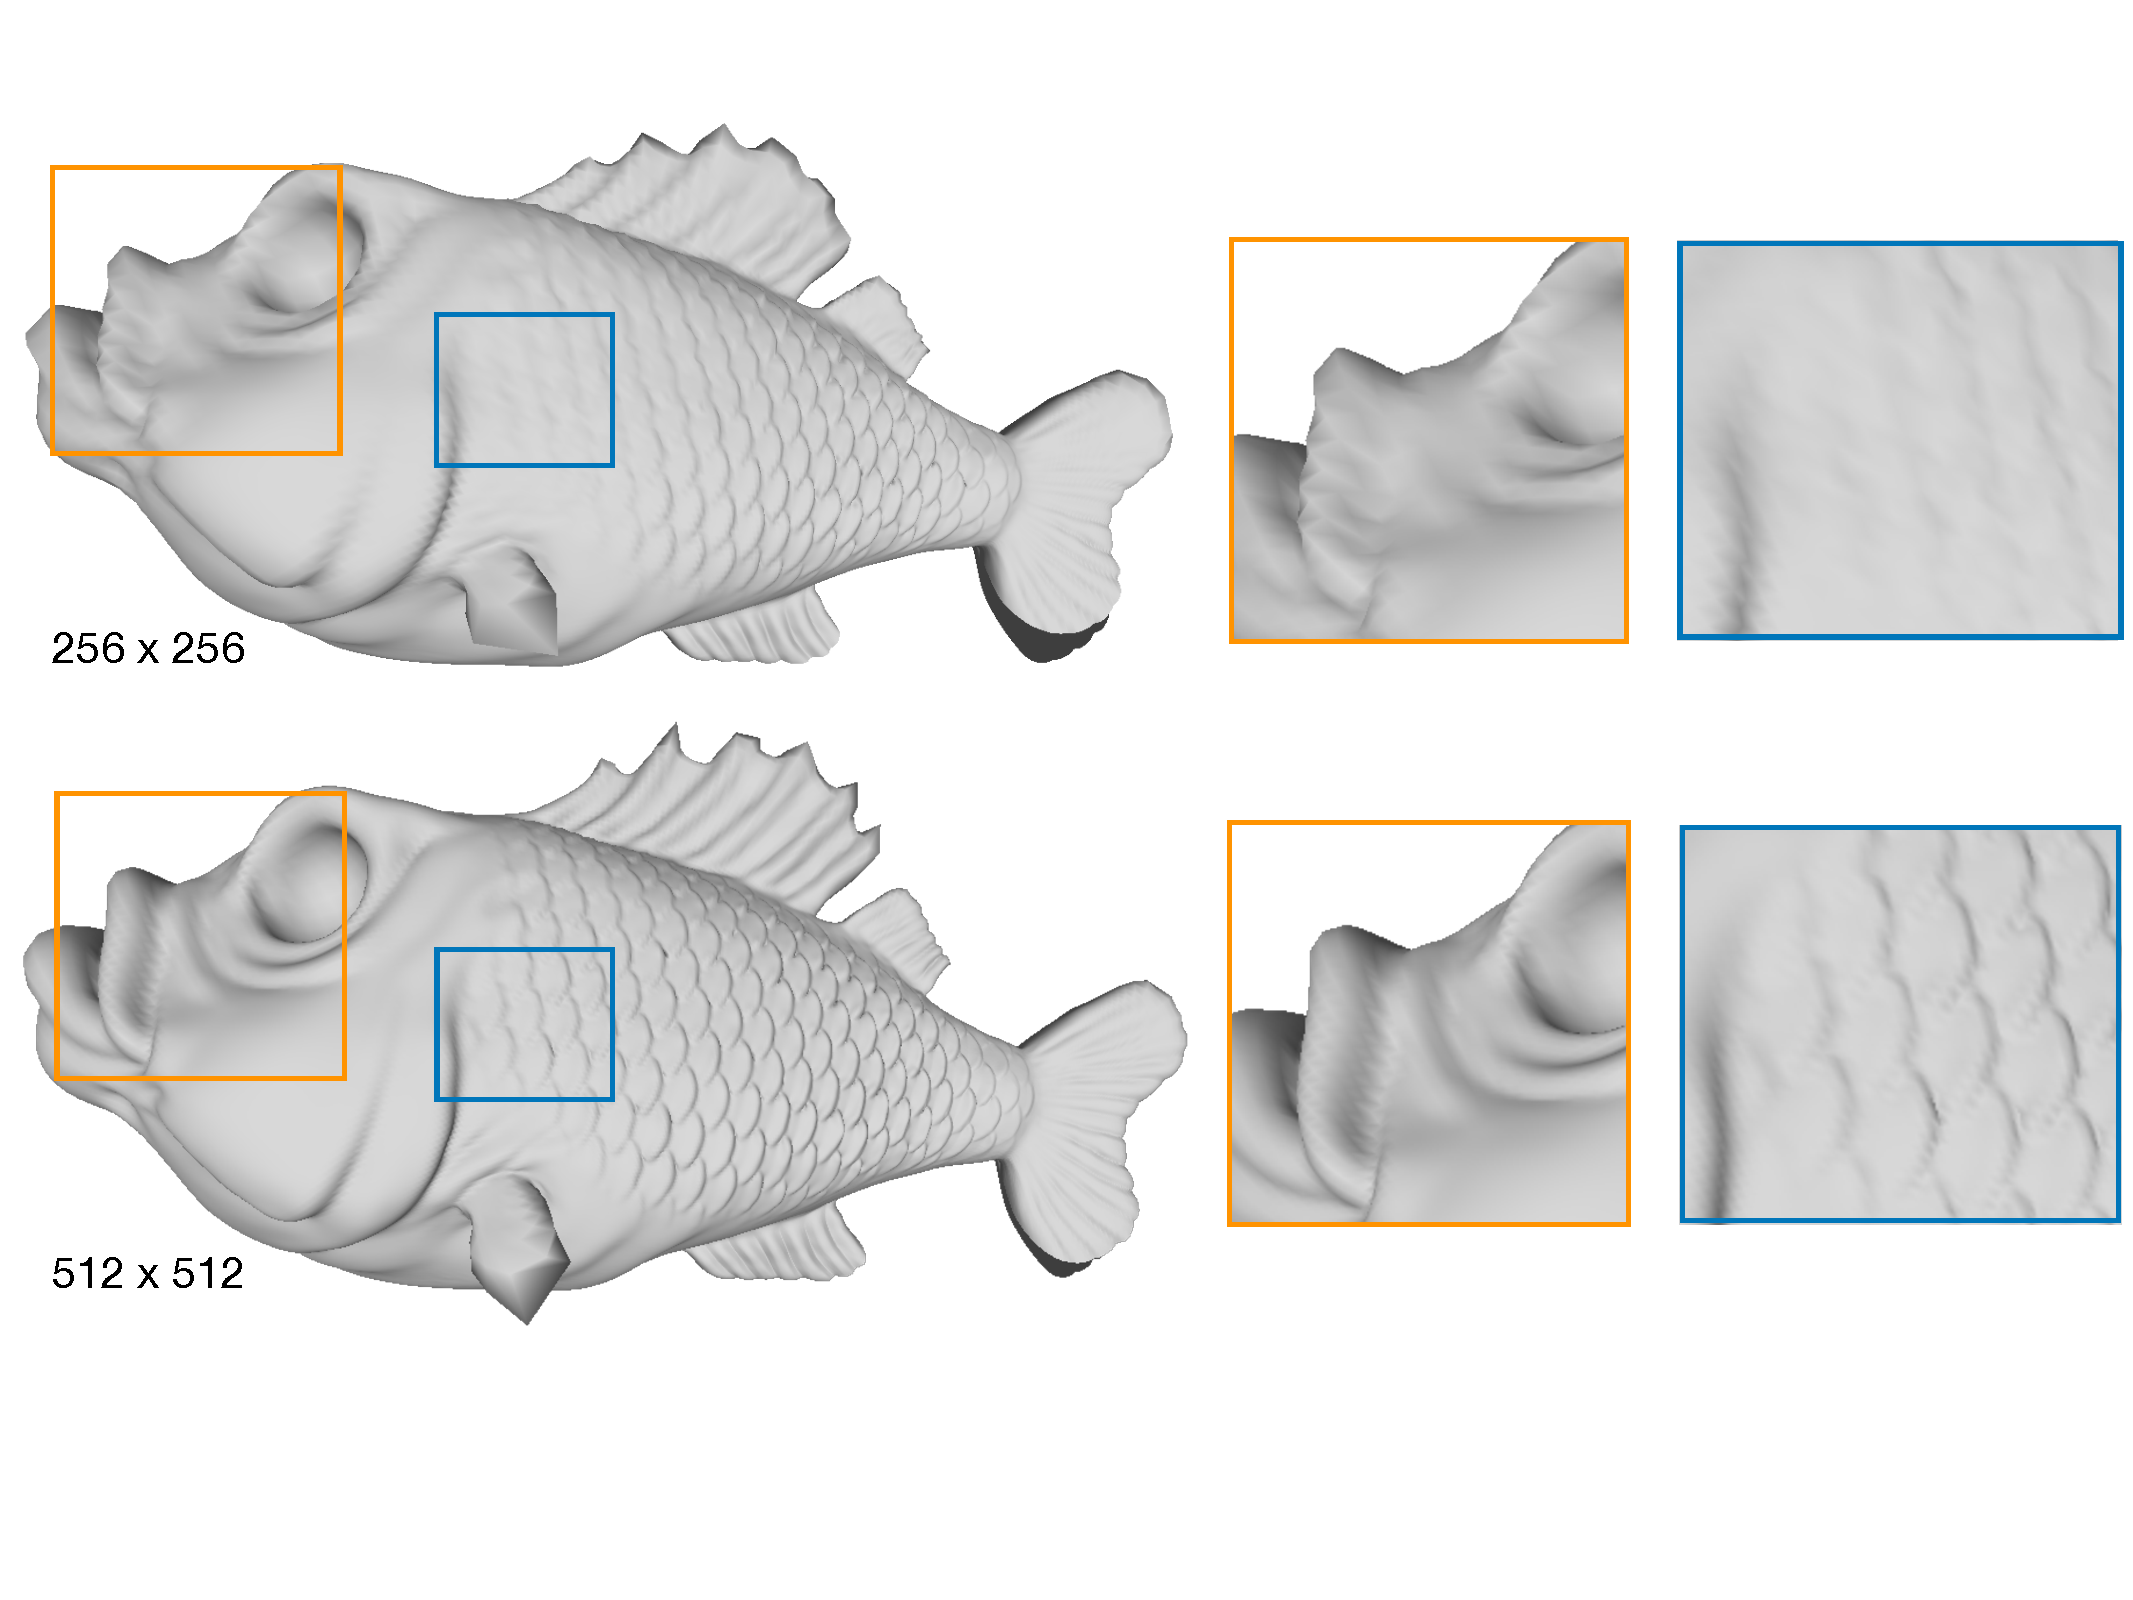
\includegraphics[width=0.5\textwidth]{Figures/fish}
     \caption{Fish reconstructions after uniform-resampling of Harmonic Map}
     \label{Fig: Fish Reconstruction}
\end{figure}
%%%%%%%%%%%%%%%%%%%%%%%%%%%%%
% CMEMORY and QUALITY
%%%%%%%%%%%%%%%%%%%%%%%%%%%%%
\subsection*{Memory Savings}
For each of the test objects, our training sets comprises 450 distinct object deformations. \\
Now, for demonstration purposes, lets assume the shapes of this training set are precisely the target shapes which appearances are requested to be computed for a given application.
\\
Within that training set, our CNN model is able to achieve accuracies up to 98\% (table \ref{Table: NN_Accuracy}) and its rendered appearances become visually indistinguishable from the ground truth (Figure (\ref{Fig: DPRT_Quality}) ). 
This means, that our trained network is able to faithfully generate self-shadowing effects of 450 distinct shapes \textbf{at the very least}, only requiring the storage of the network parameters.
\\ 
On the contrary classic PRT would imply storing the transfer coefficients of each vertex for every single shape of the training set.
\\ 
For our particular network of approx. $11,8$ million parameters,  the example objects with $256 \times 256$ and $512 \times 512$ number of vertices, and  a choice of 16 transfer coefficients per vertex, this implies a compression ratio of: 
\begin{align*}
r = \frac{\text{\# PRT-params}}{\text{\# CNN-params}}  = 
\begin{cases}
\textbf{40,022} , & \mbox{for } 256^2 \mbox{ \#vertices} \\
\textbf{160,088} & \mbox{for } 512^2 \mbox{ \#vertices}
\end{cases}
\end{align*}
This number grows linearly with increasing number of coefficients, number of deformations or number vertices. 
%%%%% TABLE %%%%%%%%%%%
\begin{table}[H]
\begin{tabular}{|l|l|l|l|l|}
\hline
\textbf{}            & \textbf{Accuracy} & \textbf{Loss} & \multicolumn{2}{l|}{\textbf{Val-Loss}} \\ \hline
\textbf{Pirate Head} & 0.9817            & 0.000397            & \multicolumn{2}{l|}{0.000399}                 \\ \hline
\textbf{Fish}        & 0.9729            & 0.002104            & \multicolumn{2}{l|}{0.002200}                 \\ \hline
\textbf{Cloth}       & 0.9818            & 0.000786            & \multicolumn{2}{l|}{0.000907}                 \\ \hline
\end{tabular}
\caption{Network Accuracy}
\label{Table: NN_Accuracy}
\end{table}
%%%%%%%%%%%%%%%%%%%
The numbers shown above express the compression ratio taking into account solely the training set. On top of that, our network shows good generalisation properties, also enabling accurate and qualitatively precise appearance predictions of deformations outside the training set. Thus, by taking this into account the compression ratio grows to immeasurable values. 
\\
Thus, we show that DPRT, as it is, is capable of drastically diminishing the storage consumption of PRT algorithms for deforming objects. 
\\
As mentioned above, commonly deep convolutional networks itself can be highly optimised, hence making DPRT even much more efficient, energy, speed and memory wise \cite{Survey_NN_Compression}. 
%%%%%%%%%%%%%%%%%%%%%%%%%%%%%
% Comparisson 
%%%%%%%%%%%%%%%%%%%%%%%%%%%%%
\subsection*{Generality of DPRT and Comparison}
\subsubsection*{Generalisation Capability:}
We validate the generalisation capabilities of our model by standard machine learning procedures. We base our parameter tuning on minimising the validation loss and later analyse prediction quality using a test set.\\ 
The results show small errors and are in most cases visually indistinguishable or close to the ground truth (Figure [??]). 
\begin{figure}[H]
  \centering
    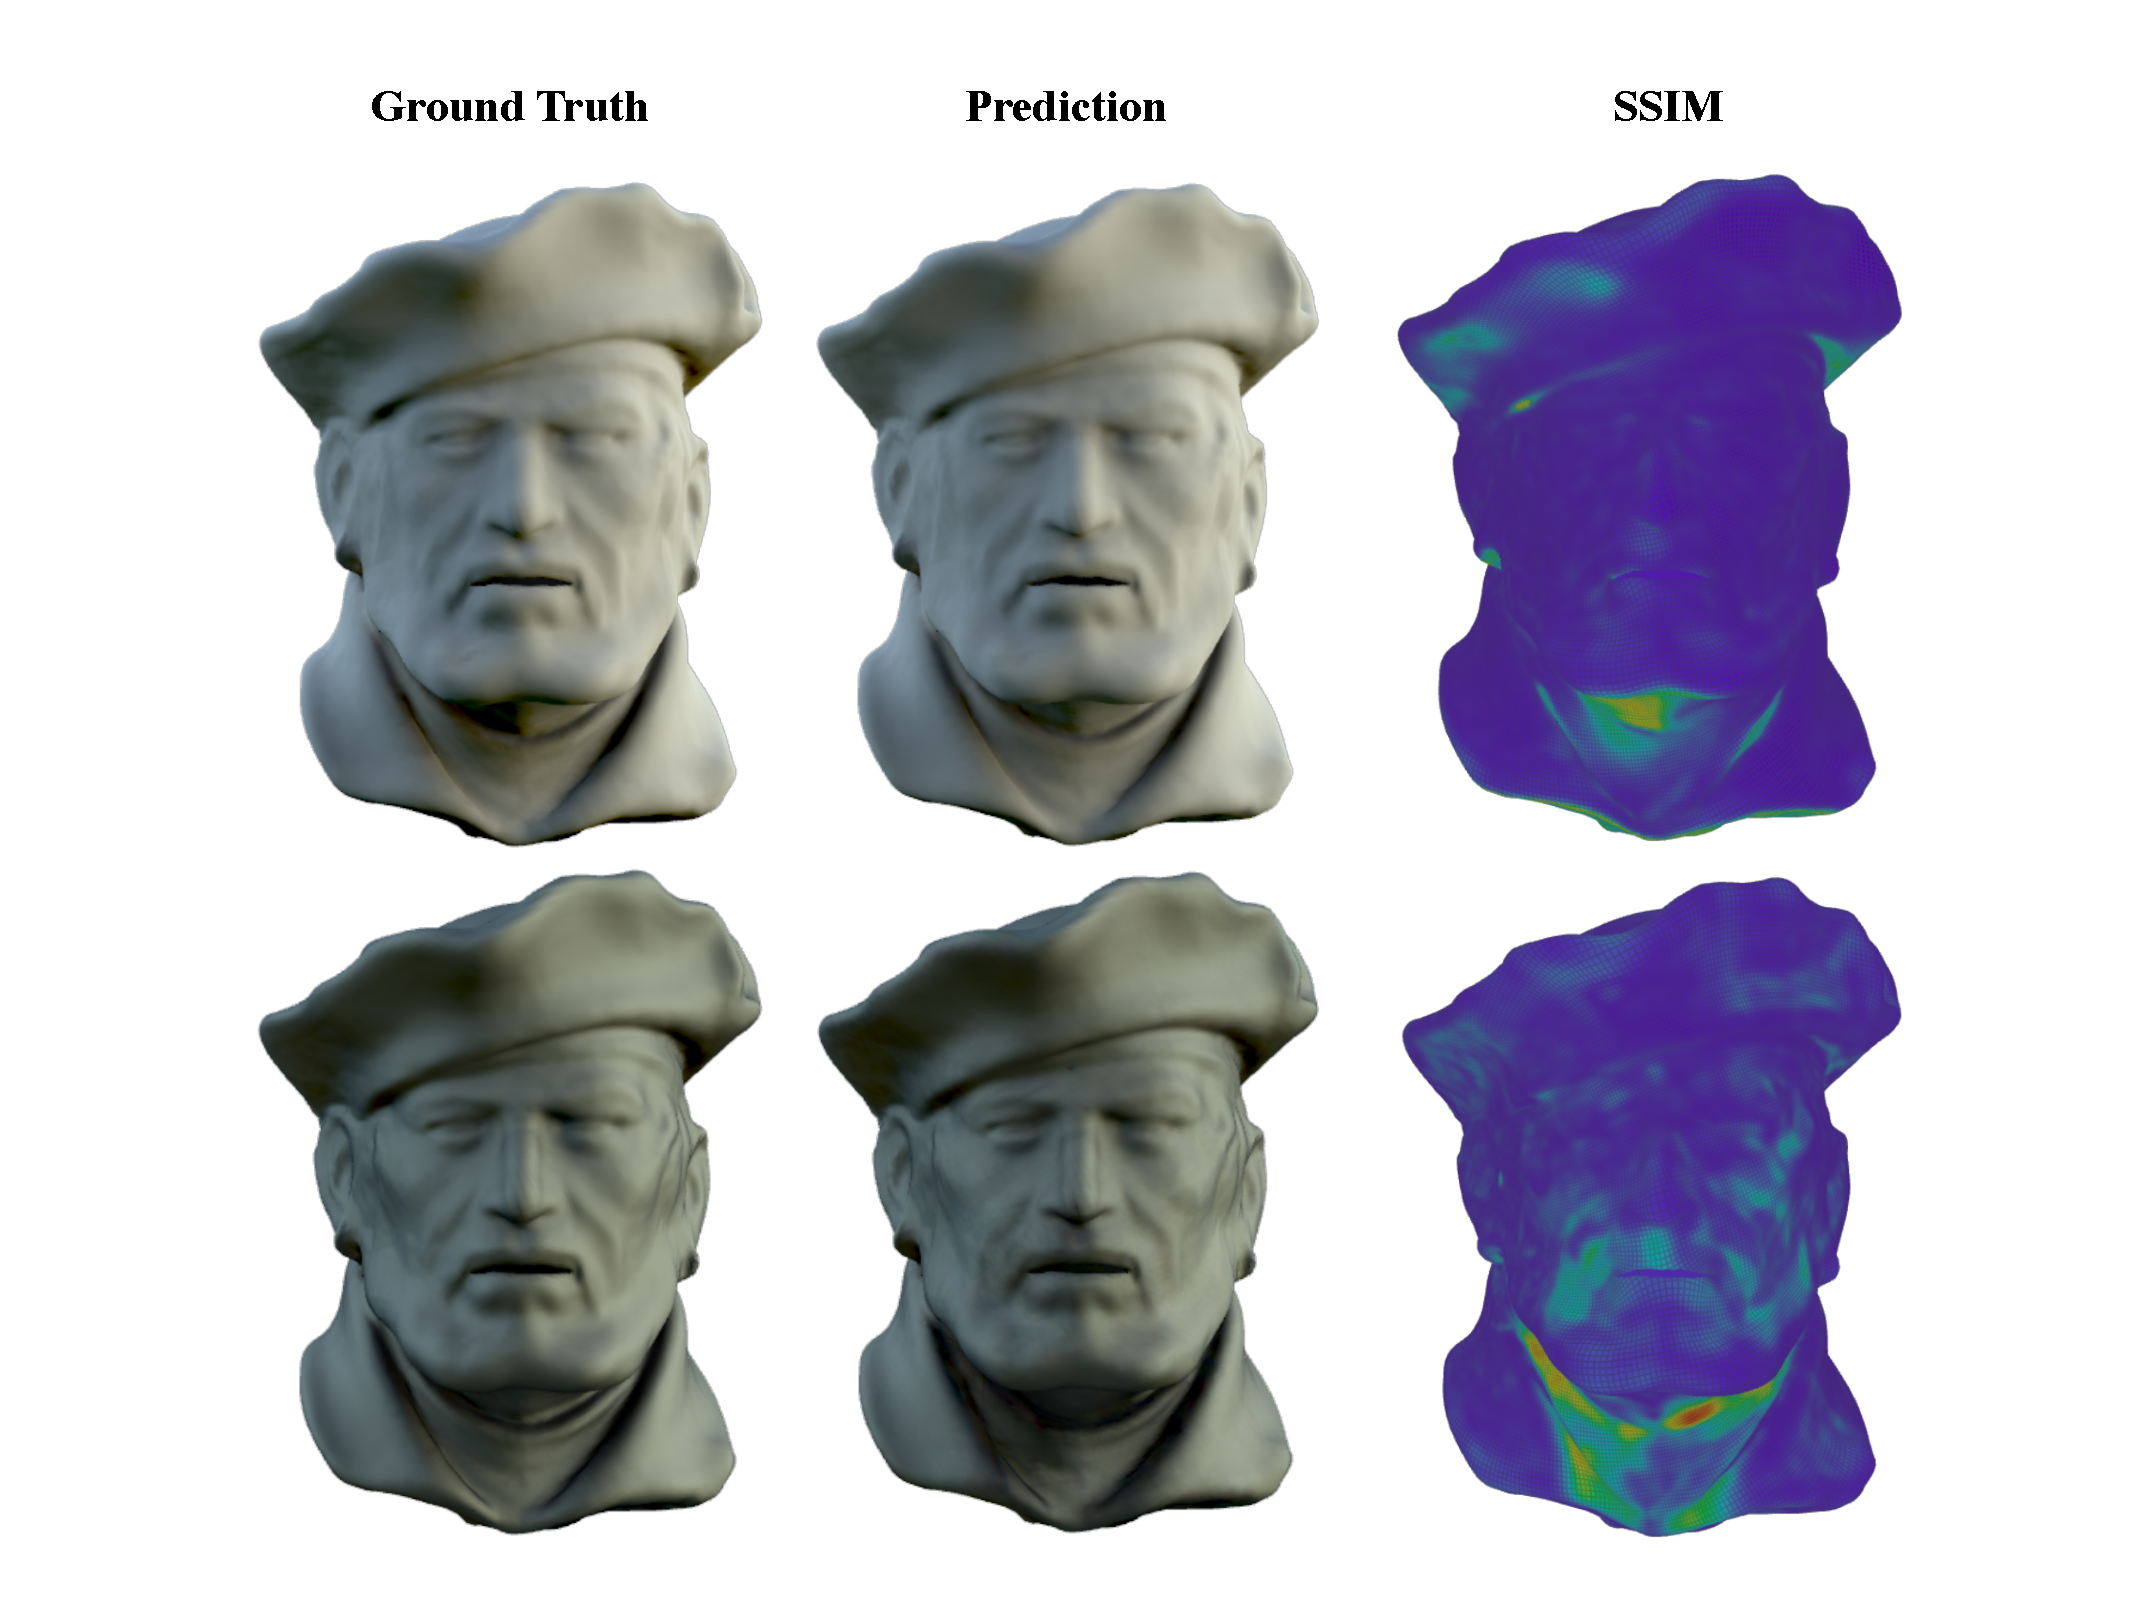
\includegraphics[width=0.35\textwidth]{Figures/glossy_pirate.pdf}
     \caption{Example: glossy pirate}
     \label{Fig: glossy_pirate}
\end{figure}
\subsubsection*{\textbf{Comparison with MoMoPRT}~:}
Furthermore, we compare our method with \cite{MoMoPRT} (MoMoPRT) and show that DPRT it is more accurate and can handle more general deformations. \\
The authors of \cite{MoMoPRT} proposed a linear model $f_{lin}$ to predict transfer coefficients within a "linear shape space", namely the space spanned by a Morphable Model.\\
This approach is clearly limited to shape deformations that are contained within the space described by the linear-shape-model $S_{lin}$ of choice. Moreover, although a linear model may be enough to approximate self-shadowing effects of shapes that are close to the mean shape of the training-data-distribution, the model lacks complexity to accurately approximate data samples that exist farther away from the mean shape (underfitting).  
\\
On the other hand, our more complex non-linear CNN model ($f_{CNN}$) is able to capture the relationships between the dataset's features (shape) and the target variable (transfer coefficients), enabling accurate approximations for a much larger deformation domain.\\
\\
For demonstration purposes, we generate a new training set consisting of, randomly sampled, linear combinations between visually more dissimilar basis shapes\footnote{More distinguishable between each other, than between each face expressions used in \cite{MoMo}.}: 1) the \textit{Pirate Head } on one side, and 2)  a simple \textit{Plane} on the other. We train both models, $f_{CNN}$ and $f_{lin}$, and compute their predictions for a series of test-shapes that are evenly distributed over the linear shape space. Figure (\ref{Fig:DPRT vs MoMoPRT A}) shows that the prediction accuracy of our $f_{CNN}$ model is higher and remains almost constant over the entire domain; on the contrary, the prediction accuracy of the linear model $f_{lin}$ drops significantly moving away from the mean shape (the \textit{Pirate/Plane} hybrid), as expected. 
\begin{figure}[H]
  \centering
    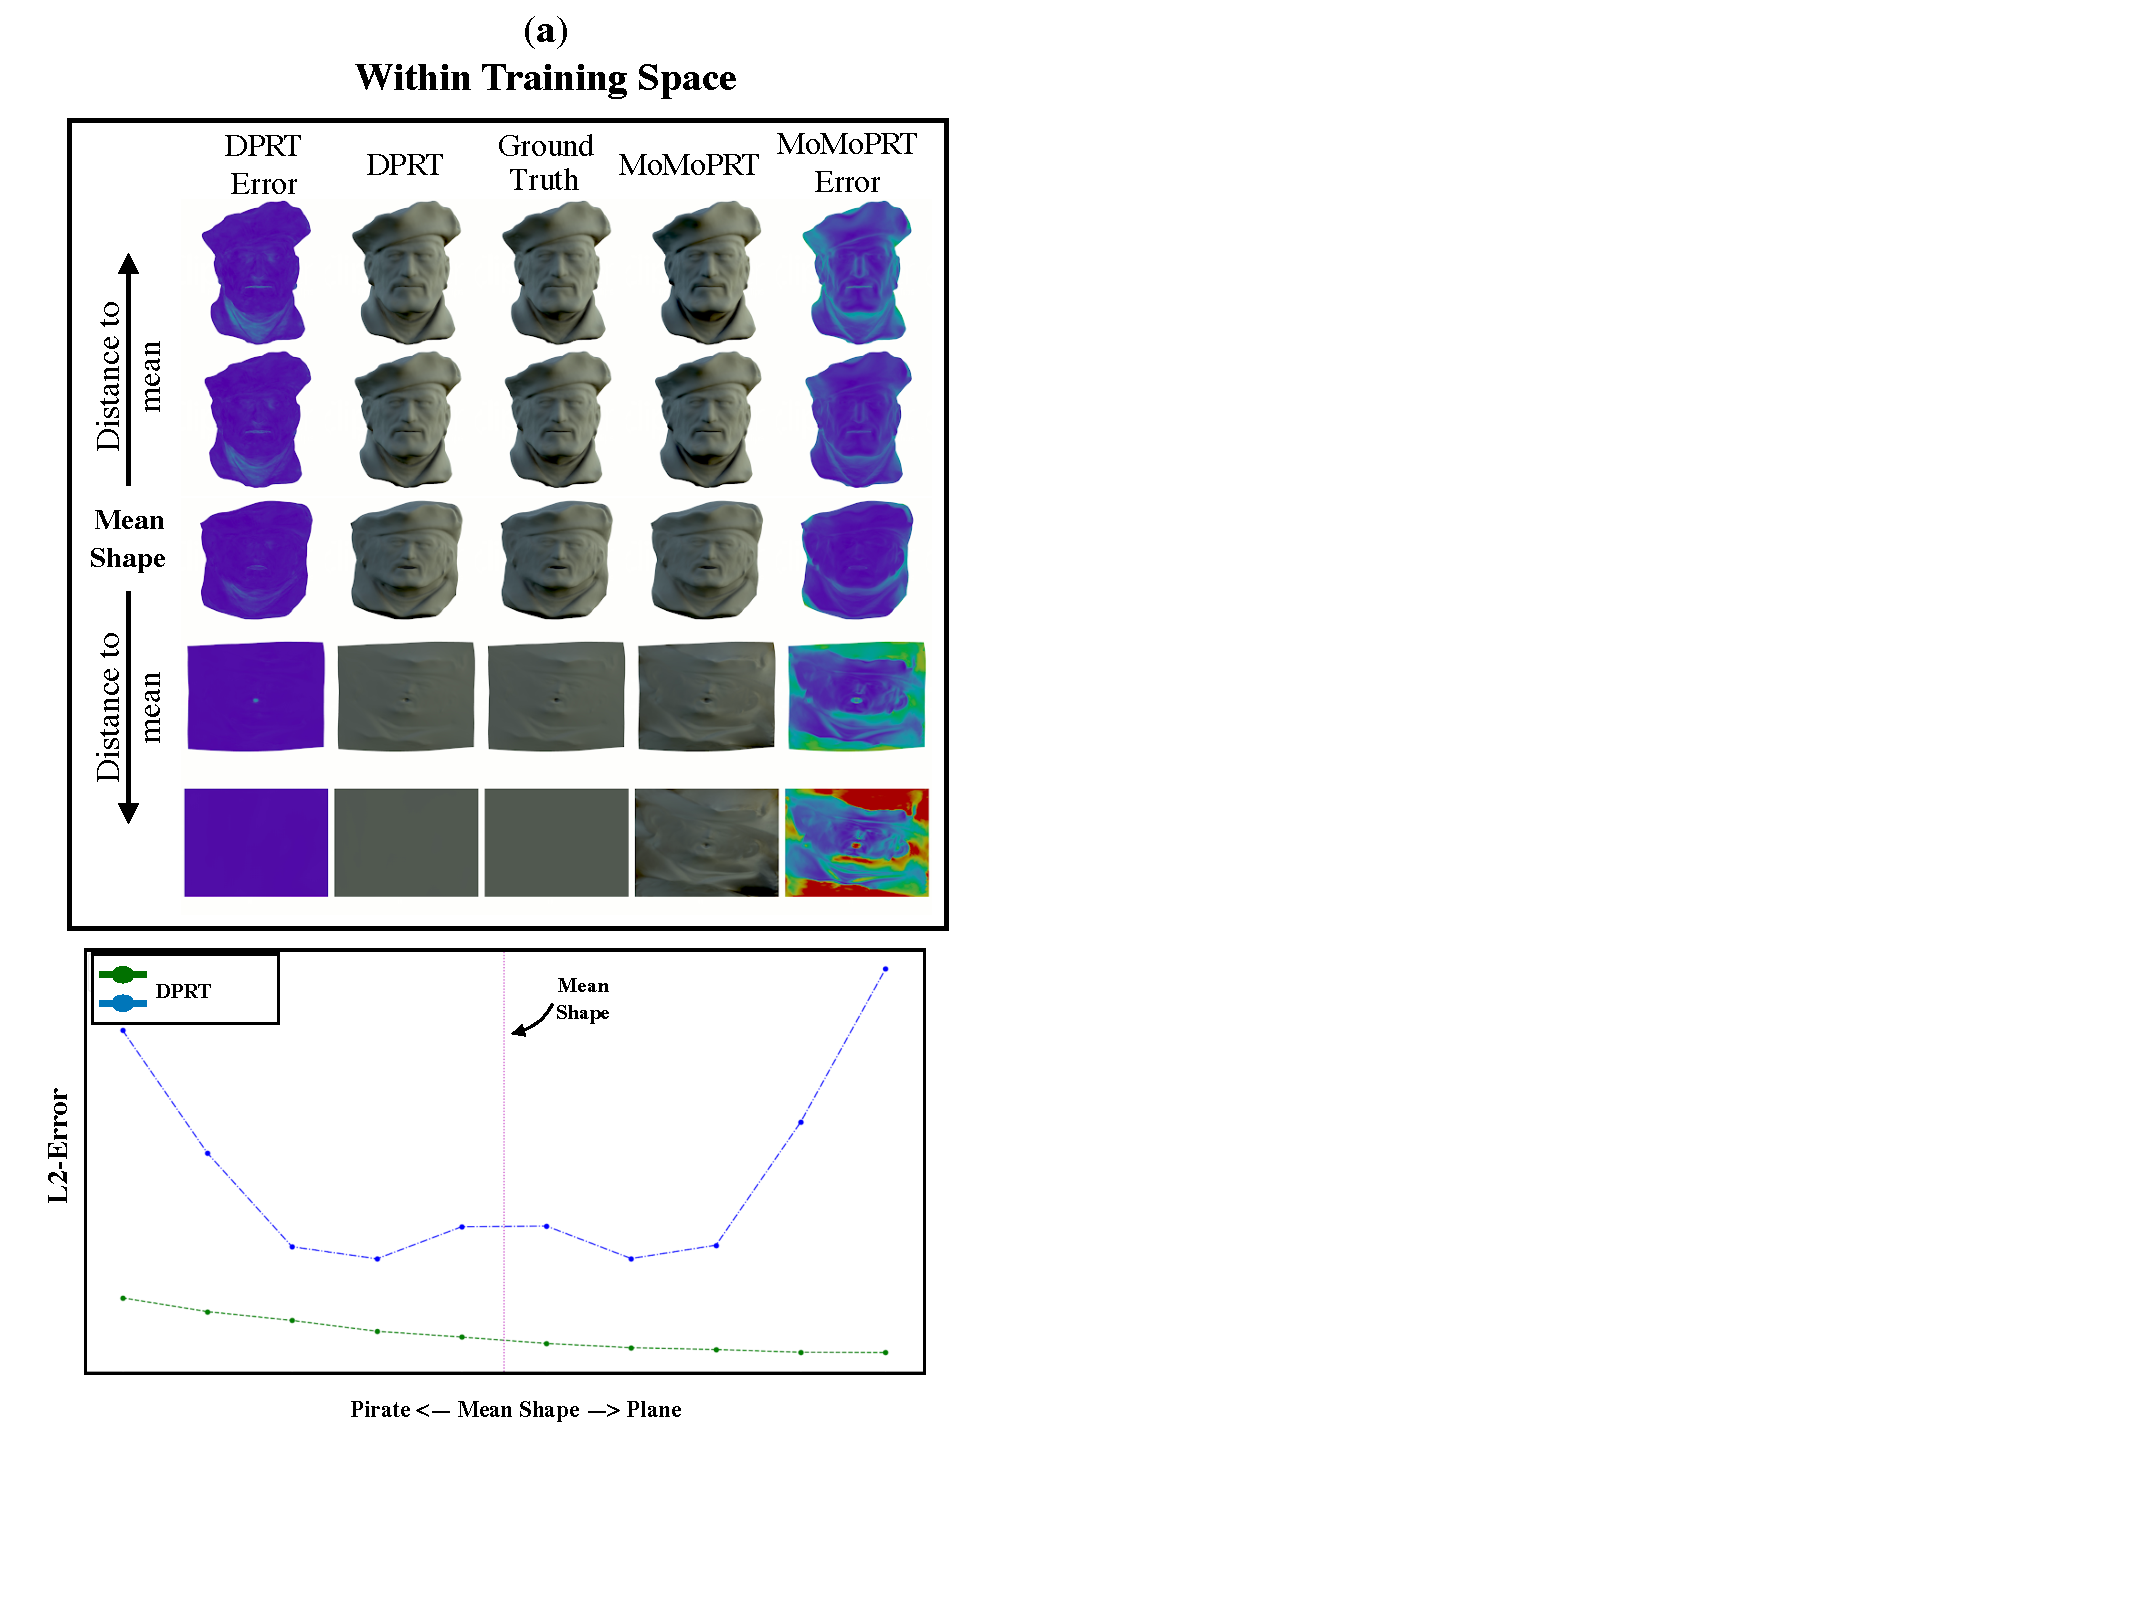
\includegraphics[width=0.5\textwidth]{Figures/DPRT_vs_MoMoPRT_a.pdf}
     \caption{Example: DPRT vs MoMoPRT}
     \label{Fig:DPRT vs MoMoPRT A}
\end{figure}
Last but not least, we demonstrate that our model approximates data that is contained in a much larger domain than the one spanned by a linear-shape-model $S_{lin}$. The models, $f_{CNN}$ and $f_{lin}$, are fed with a series of sample shapes, starting from the mean shape and increasingly deforming towards a \textit{Pirate} face expression that was excluded from the training set. \\
As can be seen in Figure (\ref{Fig:DPRT vs MoMoPRT B}), the linear model is not able to predict shapes away from its shape-space $S_{lin}$, while our method, again shows a close to constant prediction accuracy.
\begin{figure}[H]
  \centering
    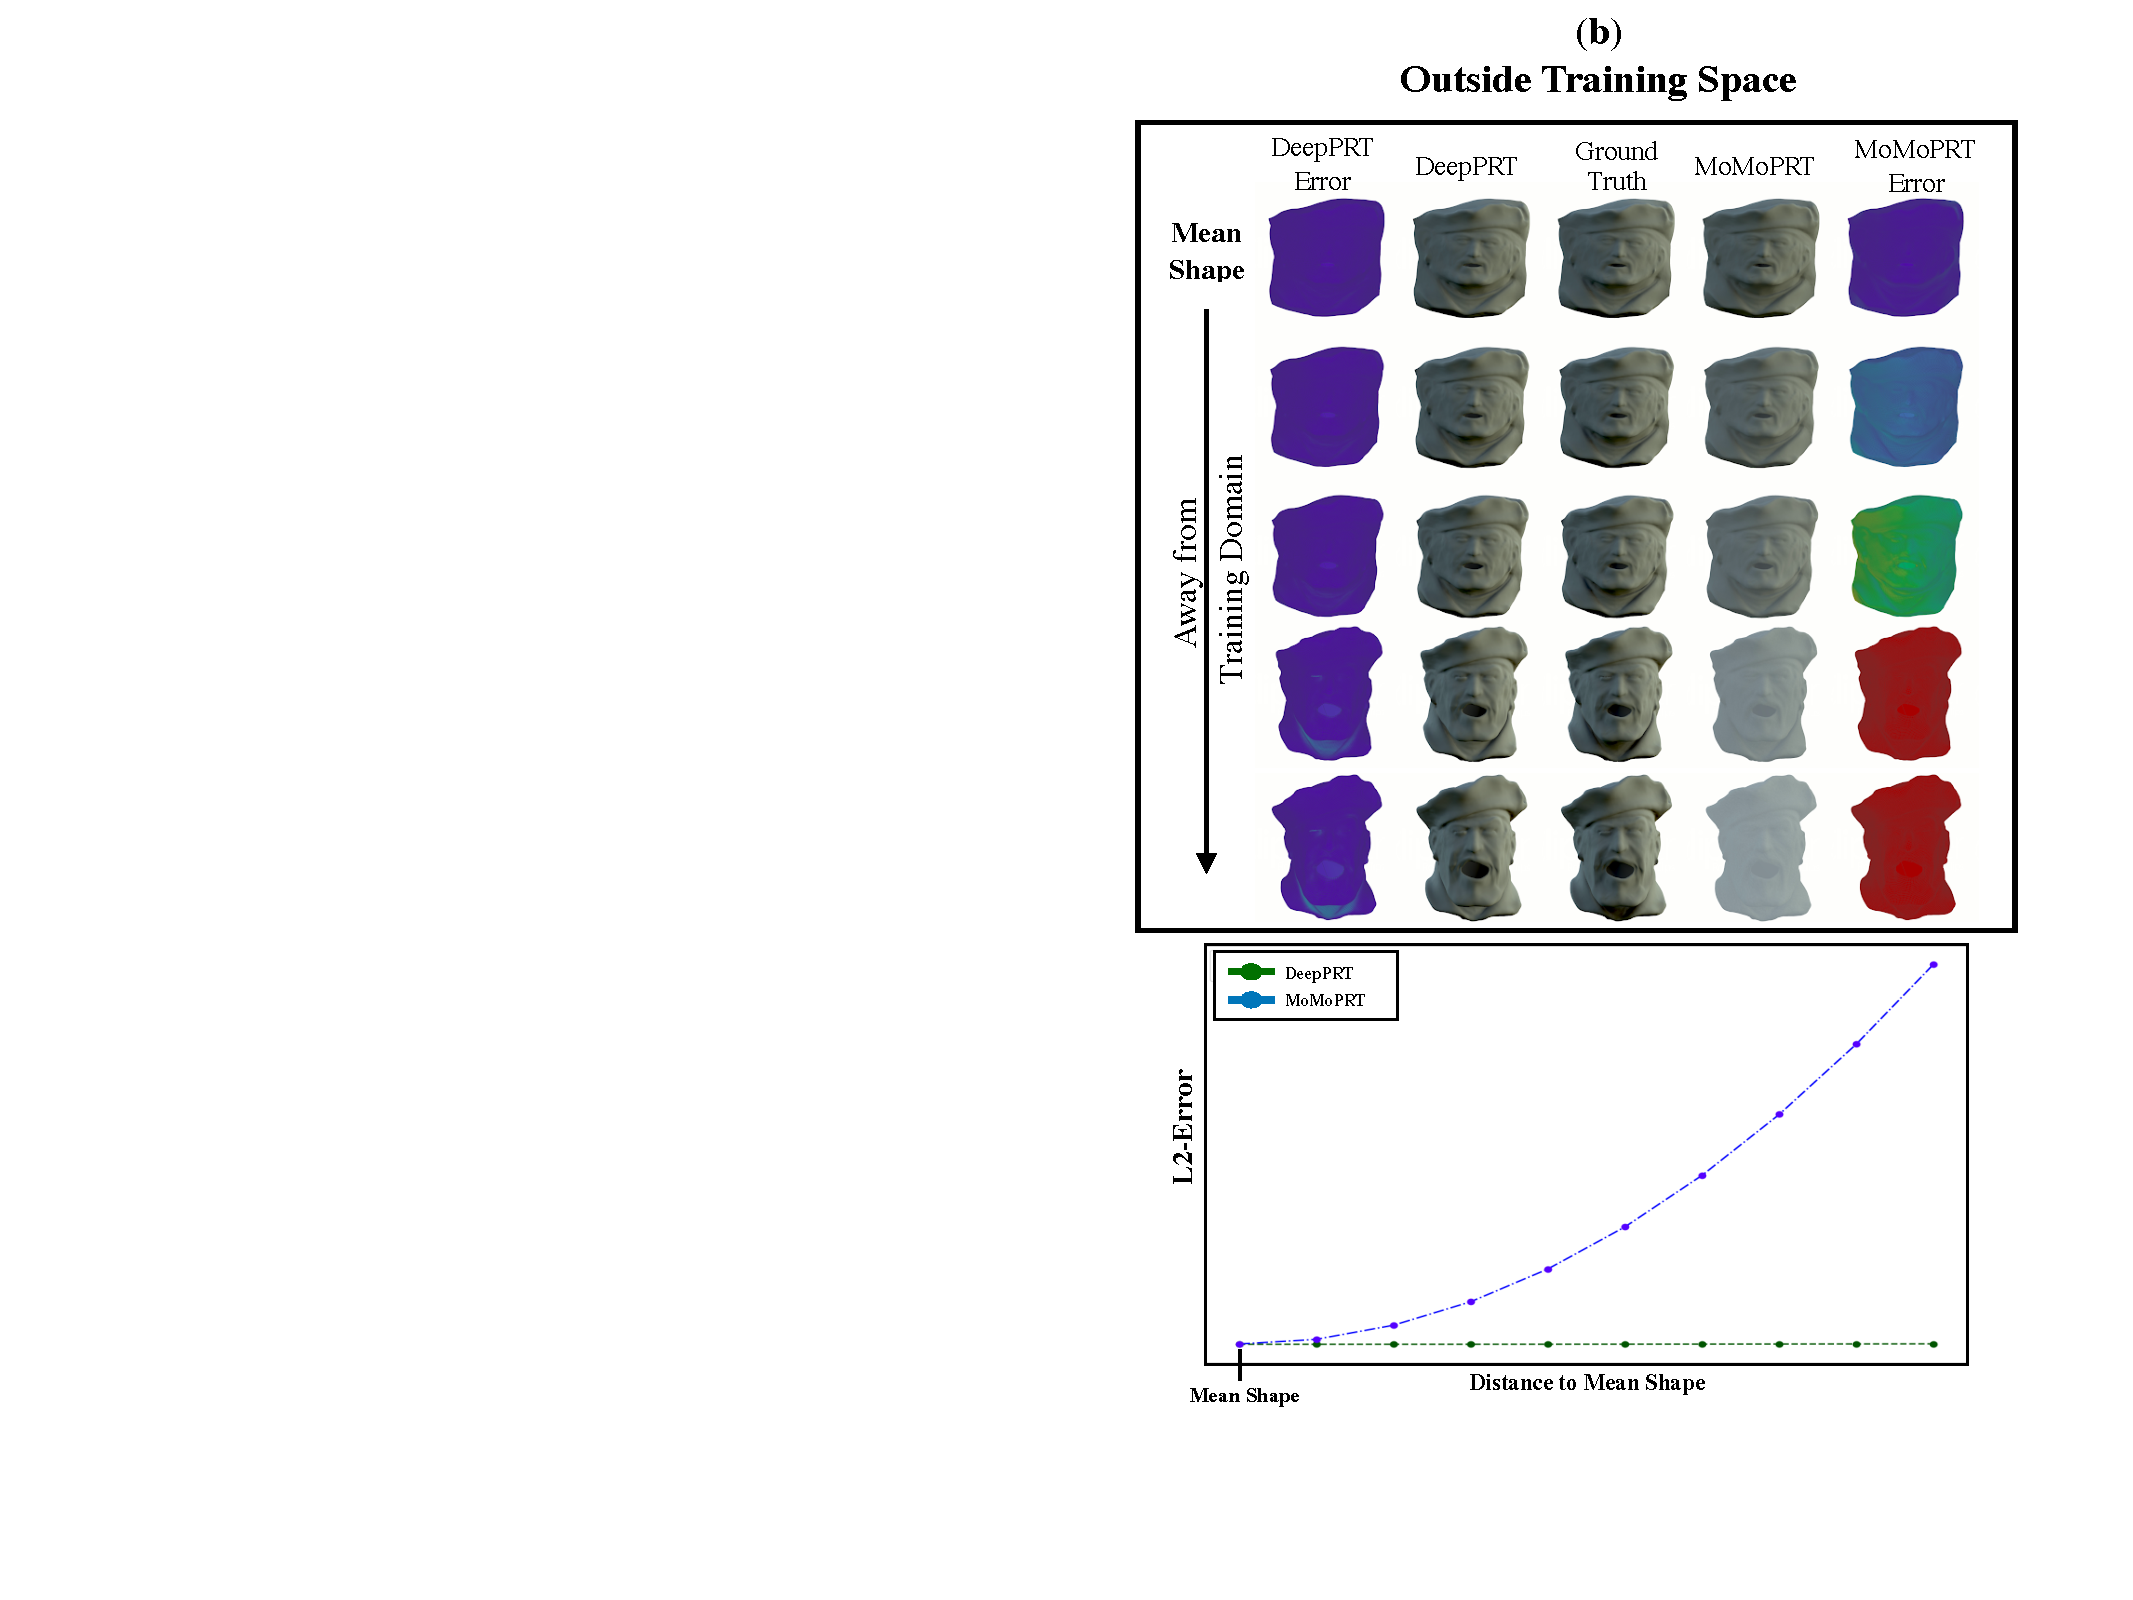
\includegraphics[width=0.45\textwidth]{Figures/DPRT_vs_MoMoPRT_b.pdf}
     \caption{Example: DPRT vs MoMoPRT}
     \label{Fig:DPRT vs MoMoPRT B}
\end{figure}
\begin{figure*}
  \centering
    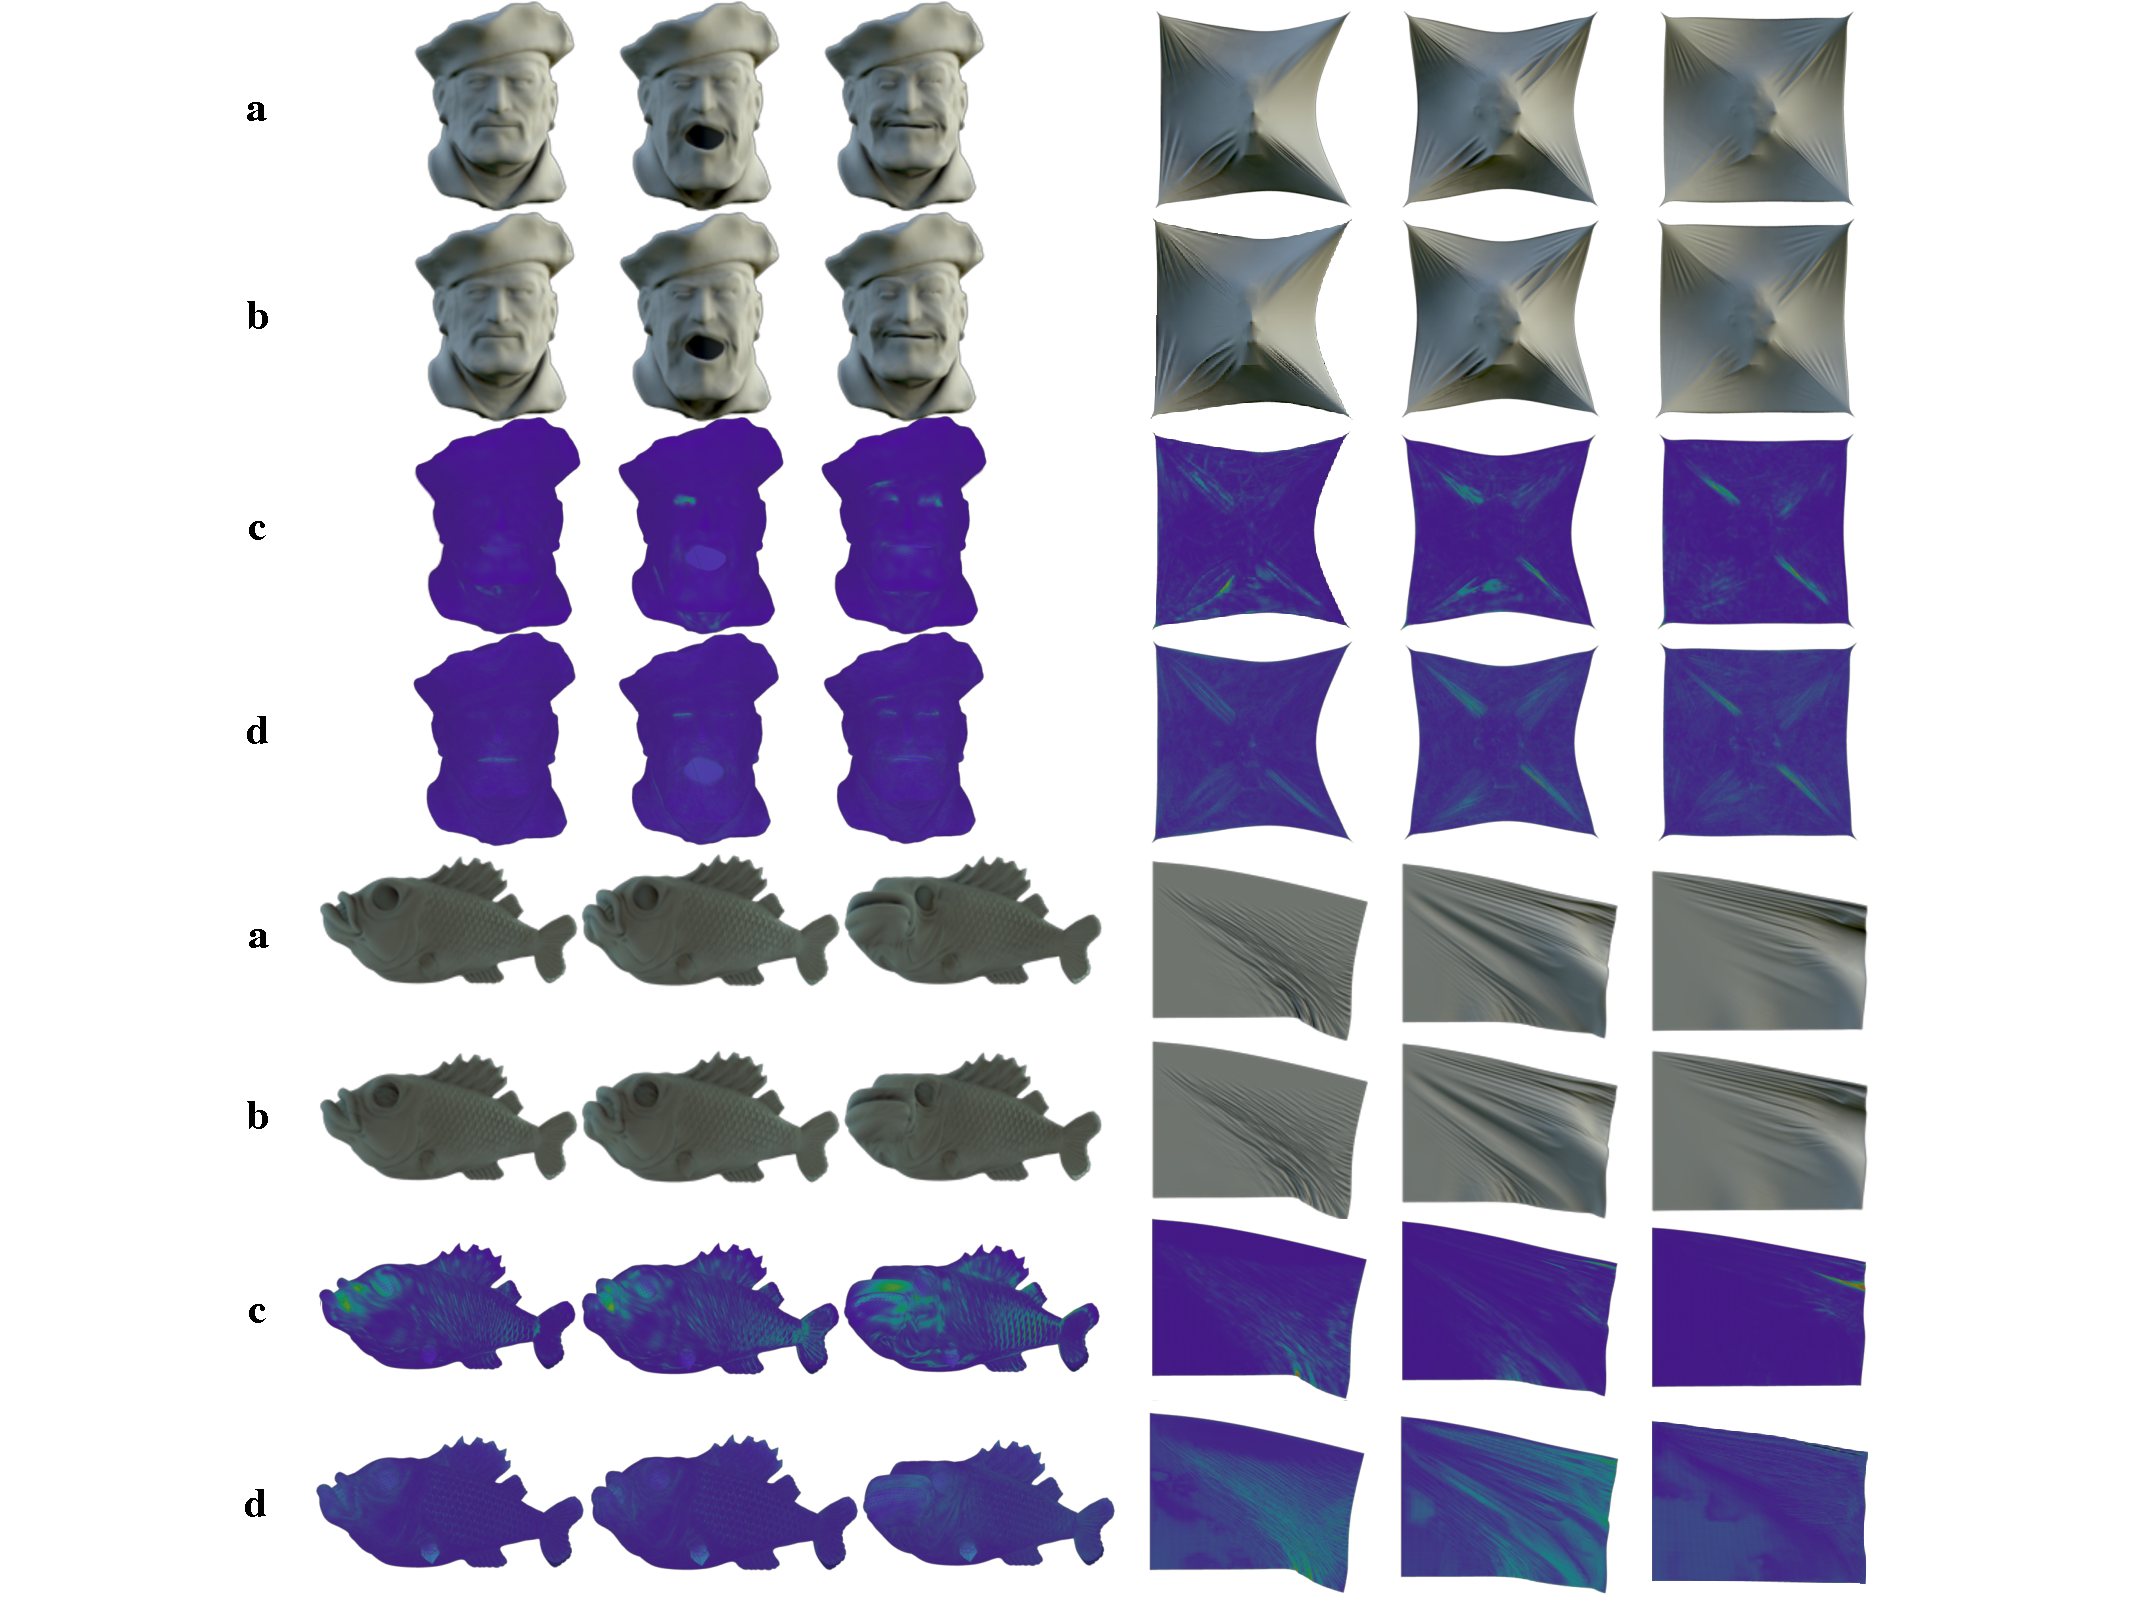
\includegraphics[width=0.8\paperwidth]{Figures/DPRT_quality_SSIM.pdf}
     \caption{Visual Quality:
     a : Ground truth appearance. b: CNN appearance prediction. c: SSIM. d: L1-Error between ground truth and predicted transfer coefficients }
     \label{Fig: DPRT_Quality}
\end{figure*}
\newpage
%
% -------- OUTLOOK -------------
\section{Conclusion and Future Work}
We present a compact representation of PRT for \textbf{free form} deformable objects, in form of a non-linear model, namely a deep convolutional neural network, with enormous memory saving potential.
 The model is able to extract the features of the dataset relevant to self-shadowing and thus generate good approximations for a wide spectrum of deformations, with resulting appearances that are visually indistinguishable from the ground truth.  
\\
Moreover, our method shows much higher generalization properties than previous approaches allowing deformations from much larger and less constrained deformation spaces.
\\
\\
Although we showed DeepPRT can be much more compact than traditional PRT, our network is far from being optimal. Exploiting network compression and acceleration methods could highly benefit DeepPRT \cite{Survey_NN_Compression}, \cite{Deep_Compression}.
Moreover, other network topologies and/or cost functions could be explored in order to achieve  better approximations, for instance, as proposed in \cite{Deformable_UNet} to account for individual object deformations the use of deformable convolutions \cite{DeformableCNN} could be investigated.
\\
The particular choice of our basis functions (Spherical Harmonics), currently restricts our method to low-frequency lightings. However, an extension to all-frequencies is possible by fitting the model to an alternative representation of the transfer function $T$, such as non-linear Wavelets \cite{AllFrequencyPRT}.
\\
The most significant limitations of our method reside within the choice of our parametrisation (harmonic map) and the natural flaws of the geometry images surface representation.  Currently, DeepPRT only performs well for modest curvature variations and is restricted to surfaces with one boundary (topological disks); however, using the geometric-stretch parametrisation instead and further using the extension proposed by \cite{Spherical_Parametrization}, the shape representation would be more robust and applicable to more general surfaces. 
%%%%%%%%%%%%%%%%%%%%%%%%%%%%% 
\begin{figure*}
  \centering
    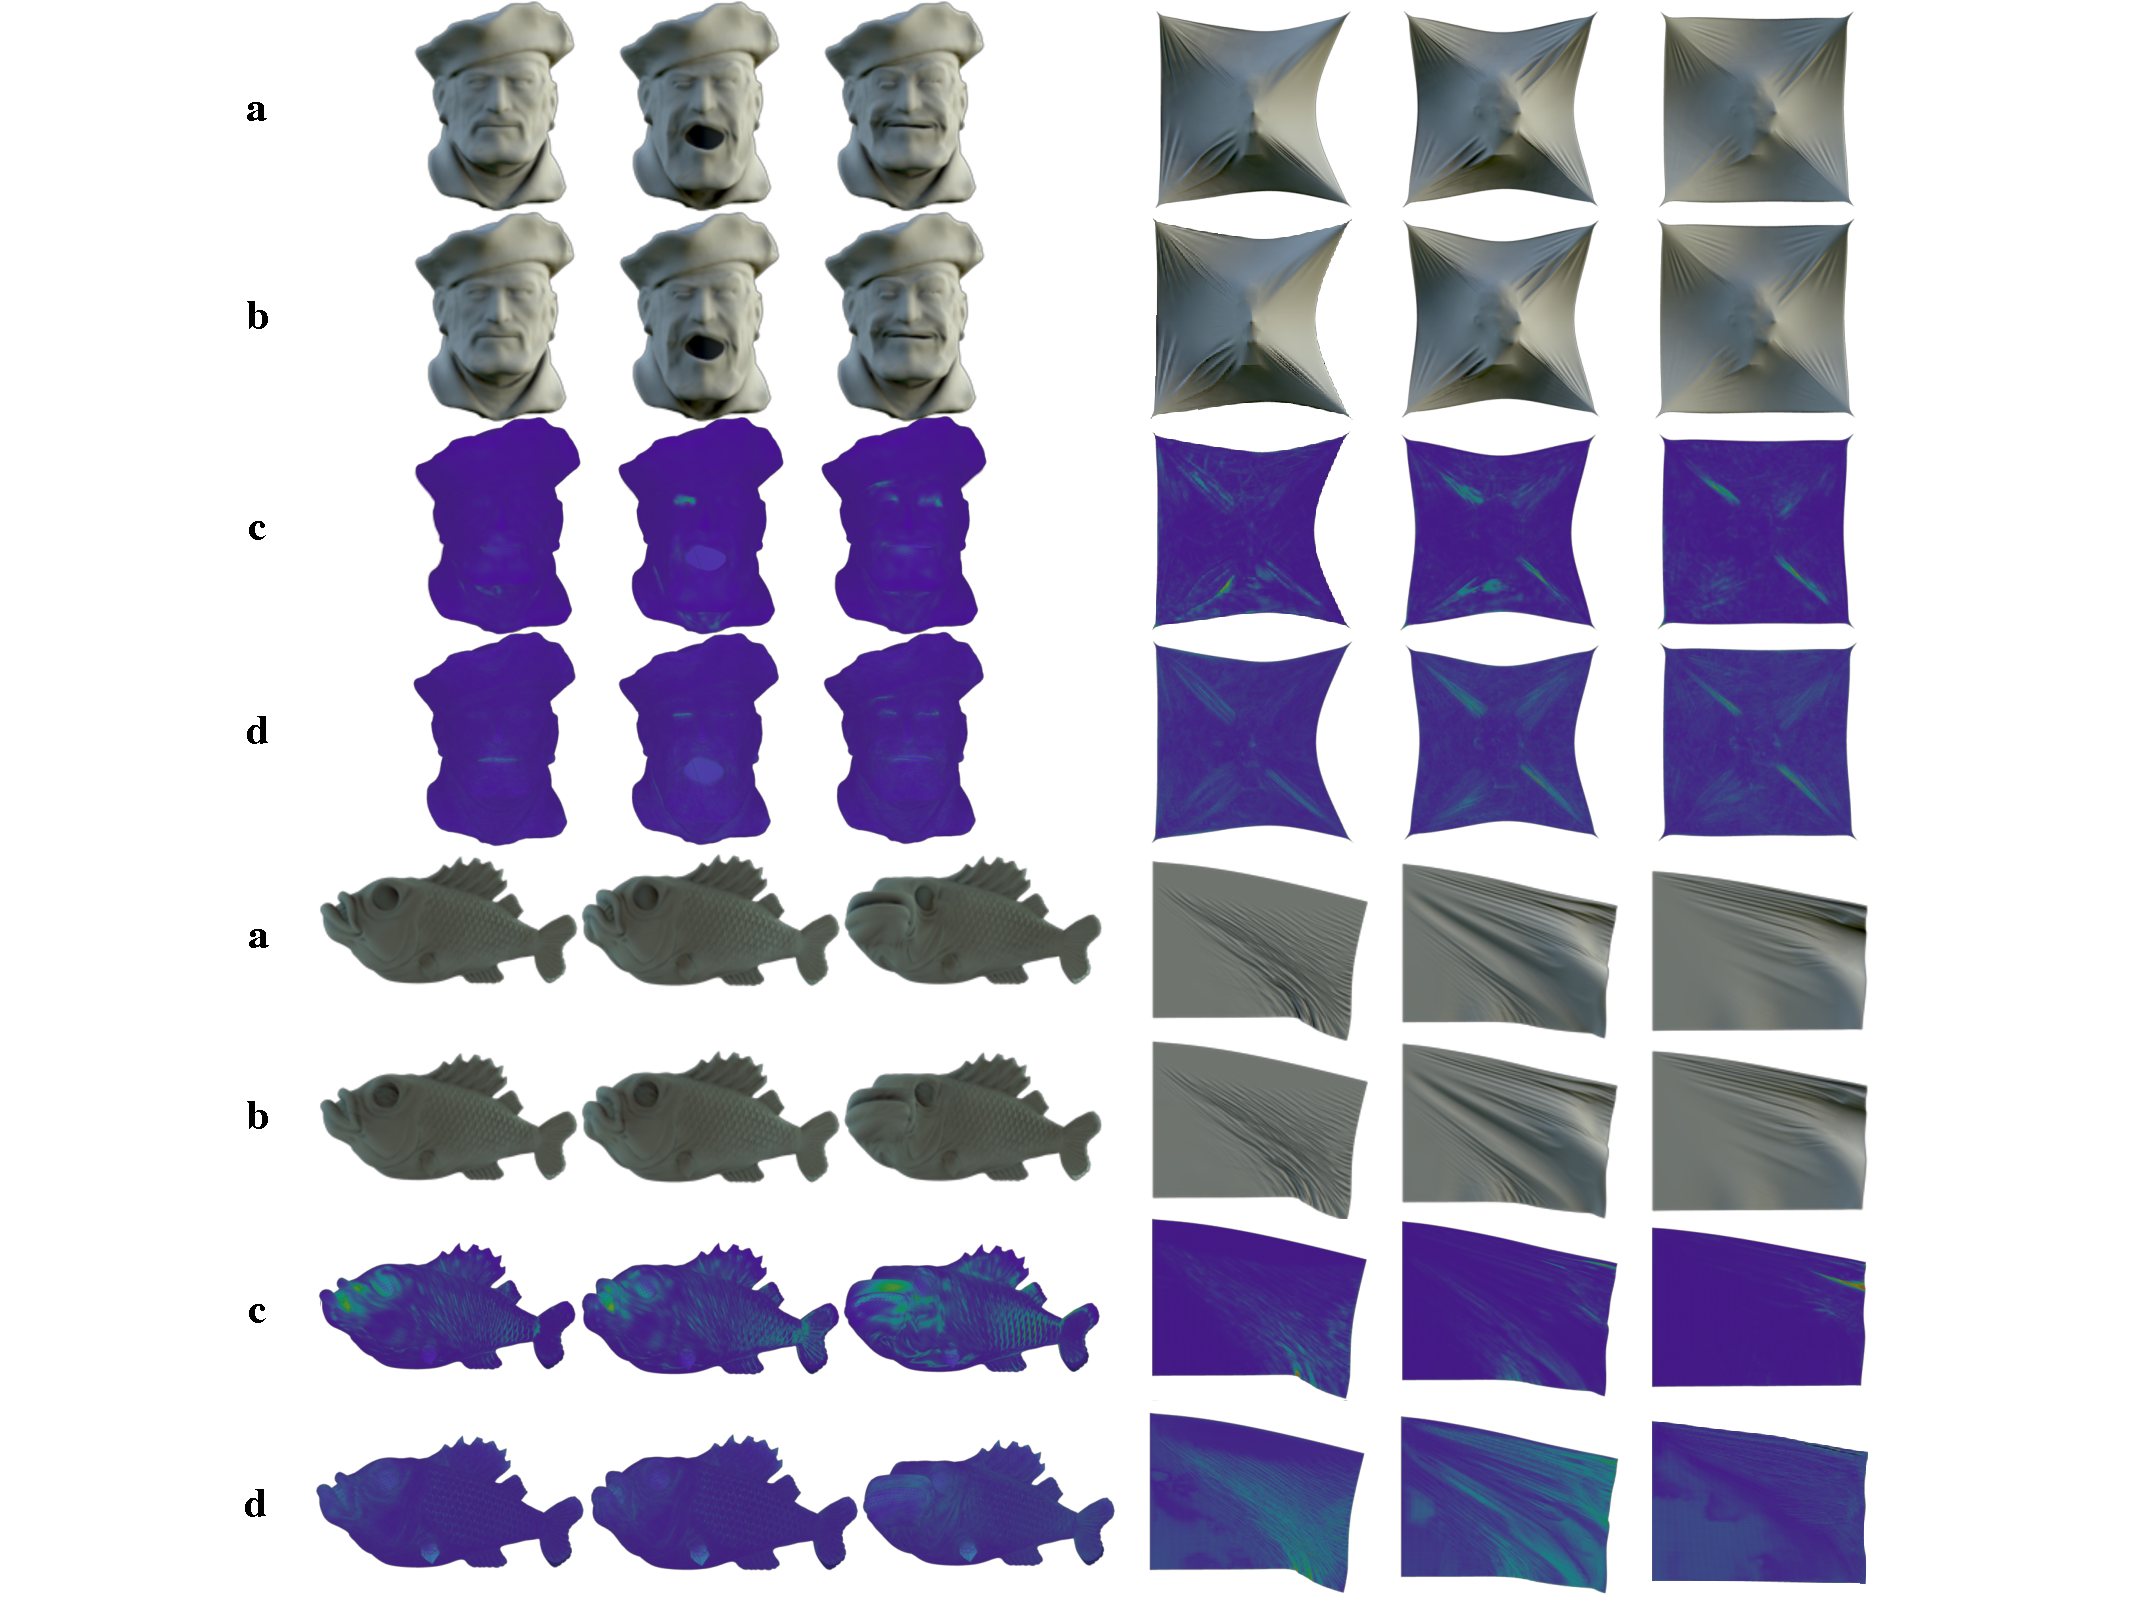
\includegraphics[width=0.7\paperwidth]{Figures/DPRT_quality_SSIM.pdf}
     \caption{Prediction Quality:
     a : ground truth appearance. b: predicted appearance. c: SSIM. d: L1-Error between ground truth and predicted transfer coefficients }
     \label{Fig: DPRT_Quality}
\end{figure*}
%
% -------- REFERENCES -------------
\newpage ~
\newpage
\bibliographystyle{ACM-Reference-Format}
\bibliography{6_ref}
%
%
\end{document}